%--------------------------------------%
%----- 3_Versuchsdurchführung.tex -----%
%--------------------------------------%
%--------------------------------------%
%
\subsection{Messung}
\label{subsec:3_Messung}
%
%------------------------------%
%----- Beginn eures Teils -----%
%------------------------------%
%
\subsubsection{Liste von Bauteile}:
\begin{itemize}
  \item Funktionsgenerator
  \item $100 \si{\kilo\ohm}$ Schichtwiderstand
  \item $1\si{\nano\farad}$ Kondensator
  \item 1 BNC-BNC Kabel
  \item $10 \si{\nano\farad}$ Kondensator
  \item 2 BNC-Doppelbananakabel
  \item Oszilloskop
  \item Steckbrett
\end{itemize}
\subsubsection{Ablauf}
Wir verbinden den $1\si{\nano\farad}$-Kondensator zunächst in Reihe mit dem Schichtwiderstand und mit dem 10nF-Kondensator. Der positive Pol der Quelle ist mit dem $1\si{\nano\farad}$-Kondensator auf dem Steckbrett und der negative mit dem $10 \si{\nano\farad}$ verbunden. Die Quelle ist auch parallel zu unserer gesamten Schaltung geschaltet. Das Oszilloskop wird parallel zum Widerstand und zum 10nF-Kondensatorzugang. Wir müssen jetzt mit dem Steckbrett auf unsere Quelle hören. Wir haben ein BNC-Doppelbananenkabel, dessen Stecker mit $V_a$ (positiver Pol) und $V_b$ (negativer Pol) verbunden sind. Jetzt müssen wir dasselbe mit dem Oszilloskop machen. Wir haben es mit dem Steckbrett durch ein BNC-Doppelbananenkabel durch $Vc$ (Pluspol) und Masse (Minuspol) gemacht. Wir müssen auch das Oszilloskop mit der Quelle verwalten. Hier haben wir ein BNC-BNC-Kabel.

Unsere Quelle sucht nach einem sinusförmigen Signal mit einer Spannung von 20 Volt von Spitze zu Spitze.

Wir müssen in unserem Versuch folgende Frequenzen betrachten:
$10,\dots,100$ (schritt:10)\\
$100,\dots,1000$ (schritt:100)\\
$1000,\dots,10000$ (schritt:1000)\\
$10000,\dots,100000$ (schritt:10000)\\
Wir haben dann $U_E$ am Channel 2 und $U_A$ am Channel 1.

In unserem Oszilloskop laufen wir mit dem Quellensignal und laufen zu horizontal/Frequenz und dann vertikal/$V_{pp}$, um die Frequenz und Spannung von $U_E$ zu messen. Wir wollen auch die Spannung von UA messen, also machen wir dasselbe für das gelbe Signal. Schließlich wollen wir den Zeitunterschied erkennen und zu horizontal/delay laufen.

Wir können jetzt anfangen zu messen. Wir notieren $U_{Epp}$, $U_{App}$, $f$ und $\Delta t$ auf.
%
%
%
\begin{flushright}
  \textit{\autorA}
\end{flushright}
%
%------------------------------%
%------ Ende eures Teils ------%
%------------------------------%
%
%
%
\subsection{Simulation}
\label{subsec:3_Simulation}
%
%------------------------------%
%----- Beginn eures Teils -----%
%------------------------------%
%
Für die Simulation wir bauen die Schaltung wie wir das im Experiment bauen, jedoch für $R_{mess}$, können wir für verschiedene Variabelen die gleiche Schaltung simulieren folgendes:
\begin{figure}[H]
  \centering
  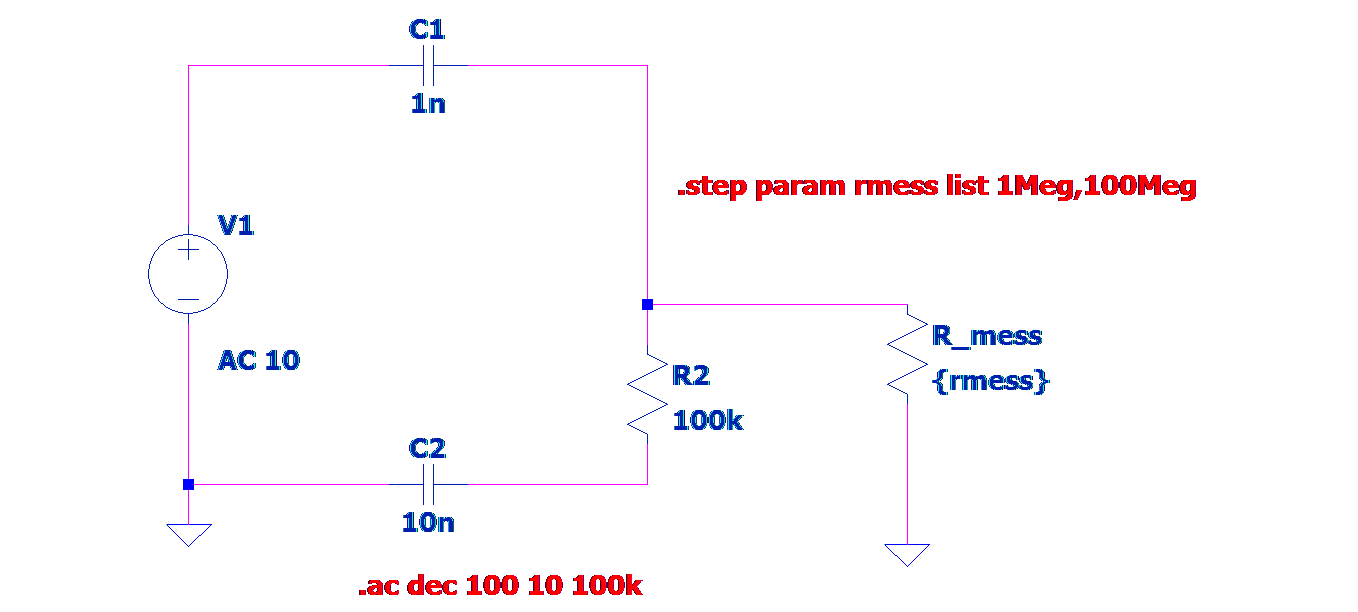
\includegraphics[scale=.4]{src/ltspice2.png}
  \caption{LTSpice schaltung}
  \label{fig:Simulationplot}
\end{figure}
%
%
%
\begin{flushright}
  \textit{\autorA}
\end{flushright}
%
%------------------------------%
%------ Ende eures Teils ------%
%------------------------------%
%
%
%